% This is a draft of the coming paper "Multiple Round Ballot Polling Risk-Limiting Audit Simulations".
% 2021.
%
\documentclass{beamer}
%
\usepackage{float}
\usepackage{xspace}
\usepackage{graphicx}
\graphicspath{{./imgs/}}
\usepackage{comment}
\usepackage{listings,hyperref}
\usepackage{cite}

% \usepackage{graphicx}  --> Used for displaying a sample figure. If possible, figure files should
% be included in EPS format.
%
% If you use the hyperref package, please uncomment the following line
% to display URLs in blue roman font according to Springer's eBook style:
% \renewcommand\UrlFont{\color{blue}\rmfamily}


% nice looking audit titles
\newcommand{\Minerva}{\textsc{Minerva}\xspace}
\newcommand{\B}{{{B2}}\xspace}
\newcommand{\R}{{{R2}}\xspace}
\newcommand{\BRAVO}{\textsc{Bravo}\xspace}

\usepackage{color}
\definecolor{green}{rgb}{0.31, 0.78, 0.47}
\newcommand{\fpo}[1]{\textcolor{green}{#1}}

\def\code#1{\texttt{#1}}

\begin{document}
\lstset{language=Python}
%
\title{Simulations of Ballot Polling Risk-Limiting Audits}
%add \thanks{} within the title brackets if want to refer to supporting organization ^^
%
%\titlerunning{Abbreviated paper title}
% If the paper title is too long for the running head, you can set
% an abbreviated paper title here
%
\author{Oliver Broadrick\inst{1} \and
Sarah Morin\inst{1} \and
Grant McClearn\inst{2}\\ \and Neal McBurnett \and Poorvi L. Vora\inst{1} \and
Filip Zag{\'o}rski\inst{3}\inst{4}}
%
% First names are abbreviated in the running head.
% If there are more than two authors, 'et al.' is used.
%
\institute{\inst{1} Department of Computer Science, The George Washington University (odbroadrick@gmail.com)
%\thanks{Supported in part by NSF Award 2015253} 
\and \inst{2} Department of Computer Science, Stanford University (grantmcc@stanford.edu)
\and \inst{3} Wroclaw University of Science and Technology (filip.zagorski@gmail.com)
%\thanks{Author was partially supported by Polish National Science Centre contract number DEC-2013/09/D/ST6/03927} and 
\and \inst{4} Votifica
}
%

%\maketitle              % typeset the header of the contribution
\frame{\titlepage}
%

\begin{frame}
\frametitle{Outline}

\begin{itemize}
\item Risk-Limiting Audits (RLAs)
\begin{itemize}
\item \BRAVO and \Minerva
\pause
\item Both are options in Arlo, statistical election audit software used by election officials across the US
\end{itemize}
\pause 
\item Experiments: simulated $10000=10^4$ audits for various margins with both
\begin{itemize}
\item a correctly announced outcome 
\item an underlying tie
\end{itemize}
\pause 
\item Observed: stopping probability, maximum risk, number of ballots
\pause 
\item Results:
\begin{itemize}
\item \Minerva requires fewer ballots over multiple rounds for both 
\begin{itemize}
\item high stopping probability (0.90)
\item low stopping probability (0.25)
\end{itemize}
\item less advantage for the lower stopping probability
\end{itemize}
\pause 
\item Discussion and Future Work
\end{itemize}

\end{frame}


\begin{frame}
\frametitle{Risk-Limiting Audits}

\begin{itemize}
\item Scanners are used to tabulate ballots
\pause 
\begin{itemize}
\item Cannot trust the machines: bugs, configuration errors, hacking
\pause 
\end{itemize}
\item Compliance and tabulation audits
\pause 
\item Risk-Limiting Audits
\begin{itemize}
\item
Given that the election outcome is incorrect,
the probability with which the audit stops, declaring the outcome correct, is at most the risk limit, $\alpha$.
\end{itemize}
\end{itemize}
\end{frame}

\begin{frame}
\frametitle{Ballot Polling Risk-Limiting Audits: A Procedure}

\begin{itemize}
\item Is a manual audit, which relies on a voter-verified paper trail and successfully completed compliance audits
\pause 
\item Sketch:
\begin{enumerate}
\item Election results announced
\pause 
\item In a public procedure, sample ballots at random and manually interpret them
\pause 
\item Compute a pre-specified error measure, the maximum risk, and compare to the risk limit
\begin{itemize}
\item If smaller, stop the audit
\item Else, sample more (goto 2)
\end{itemize}
\end{enumerate}
\end{itemize}
\end{frame}

\begin{frame}
\frametitle{\BRAVO}
\begin{itemize}
\item Most commonly used ballot polling RLA
\pause 
\item In the two candidate case is an instance of Wald's Sequential Probability Ratio Test (SPRT)
\pause 
\item Is thus the most efficient RLA when 
the decision of whether to stop the audit is made after each ballot is drawn (ballot-by-ballot)
\pause 
\item In real audits, decisions are taken after many ballots are drawn (round-by-round)
\pause 
\item \BRAVO can be implemented as:
\begin{itemize}
\item Selection-Ordered (SO) \BRAVO, 
where ballot selection order is retained, and the decisions are taken as though the audit were ballot-by-ballot
\item End-of-Round (EoR) \BRAVO, where
the decision using the \BRAVO stopping rule is taken once, after the entire round of ballots is drawn
\end{itemize}
\end{itemize}
\end{frame}

\begin{frame}
\frametitle{\Minerva}
\begin{itemize}
\item Recent RLA designed for round-by-round use
\pause 
\item \BRAVO uses the likelihood ratio; that is the ratio of points on two probability distribution functions
\pause 
\item \Minerva uses a ratio of the \emph{tails} of the pdfs used in \BRAVO
\pause 
\begin{itemize}
\item Shown to be risk-limiting if all round sizes are pre-committed, before the audit begins
\pause 
\item In a first round chosen to give a $0.90$ probability of stopping, \Minerva requires
\begin{itemize}
\item $~50\%$ as many ballots as EoR \BRAVO 
\item $~70\text{-}80\%$ as many ballots as SO \BRAVO 
\end{itemize}
\pause 
\item Unknown how the audits compare for smaller stopping probability or for rounds after the first
\end{itemize}
\end{itemize}
\end{frame}

\begin{frame}
\frametitle{Experiments}
\begin{itemize}
\item Use simulations to provide evidence for theoretical claims
\pause 
\item R2B2 software library for round-by-round and ballot-by-ballot RLAs
\pause 
\item Simulate RLAs for election results from the 2020 Presidential election (all margins above $0.05$)
\begin{itemize}
\item $10000=10^4$ trials assuming the underlying election was as announced
\item $10000=10^4$ trials assuming the underlying election was a tie
\end{itemize}
\pause 
\item Risk limit: $10\%$
\pause 
\item Round schedules:
\begin{itemize}
\item \BRAVO round sizes to achieve a chosen probability of stopping in each round given that the audit has already reached that round
\pause 
\item \Minerva first round sizes to achieve a chosen probability of stopping, and subsequent round sizes found by multiplying the previous round size by a constant ($1.5$ and $1$)
\end{itemize}
\pause 
\item Stopping probabilities: $0.90$ and $0.25$
\end{itemize}
\end{frame}

\begin{frame}
\frametitle{Experiments}
\begin{definition}
An audit $\mathcal{A}$ takes a sample of ballots $X$ as input and gives as output either
(1) $Correct$: the audit is complete, or (2) $Uncertain$: continue the audit.
\end{definition}

\pause 
\begin{itemize}
\item Binary hypothesis test: $H_0$ (a tie) and $H_a$ (announced results)
\pause 
\item The tie is the hardest incorrect outcome to detect 
\pause 
\item Probability of stopping given a tie should be low
\pause 
\item Probability of stopping given a correctly announced outcome should be high for as few ballots as possible 
\end{itemize}
\end{frame}

\begin{frame}
\frametitle{Experiments}
\begin{definition}[Maximum Risk]
The maximum risk $R$ of audit $\mathcal{A}$ with sample $X\in \{0,1\}^*$ drawn from 
the ballots is
$R(\mathcal{A})=\Pr[\mathcal{A}(X)=Correct \mid H_0].$
\end{definition}

\pause 
\begin{definition}[Risk-Limiting Audit ($\alpha$-RLA)]
An audit $\mathcal{A}$ is a Risk-Limiting Audit with 
risk limit $\alpha$ iff 
$R(\mathcal{A}) \le \alpha.$
\end{definition}
\end{frame}

\begin{frame}
\frametitle{Experiments}
\begin{definition}[Stopping Probability]
The stopping probability $S_j$ of an audit $\mathcal{A}$ in round $j$ is 
$S_j(\mathcal{A})=$
$$\Pr[\mathcal{A}(X)=Correct ~in~round~j~\land \mathcal{A}(X) \neq Correct ~previously \mid H_a]$$
\end{definition}

\pause 
\begin{definition}[Cumulative Stopping Probability]
The cumulative stopping probability $C_j$ of an audit $\mathcal{A}$ in round $j$ is $C_j(\mathcal{A})= \sum_{i=1}^j S_j$
\end{definition}

\pause 
\begin{definition}[Conditional Stopping Probability]
The conditional stopping probability  of an audit $\mathcal{A}$ in round $j$ is 
$\chi_j (\mathcal{A})=$
$$\Pr[\mathcal{A}(X)=Correct ~in~round~j~\mid H_a \land \mathcal{A}(X) \neq Correct ~previously]$$
\end{definition}
\end{frame}

\begin{frame}
\frametitle{Results: Stopping Probability ($\chi_1=0.9$)}
\pause 

\vspace{.1cm}
\hspace{-.25cm}
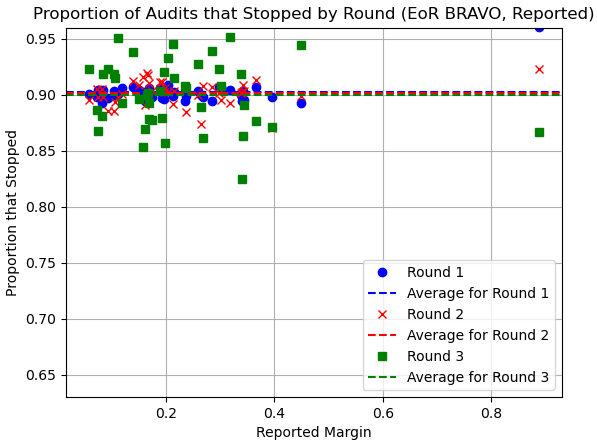
\includegraphics[width=0.5\textwidth]{scale/eor.png}
\pause 
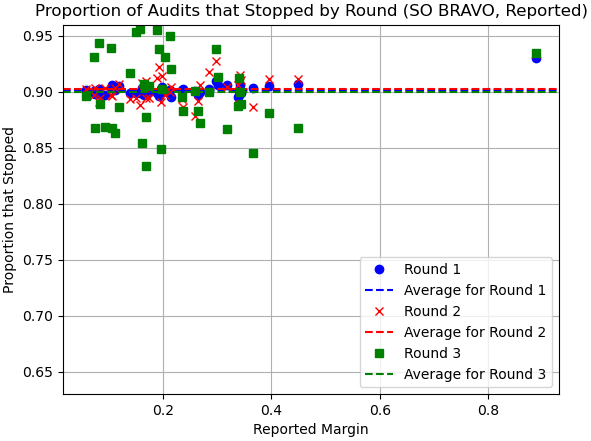
\includegraphics[width=0.5\textwidth]{scale/so.png}

\pause 

\vspace{.1cm}
\hspace{-.25cm}
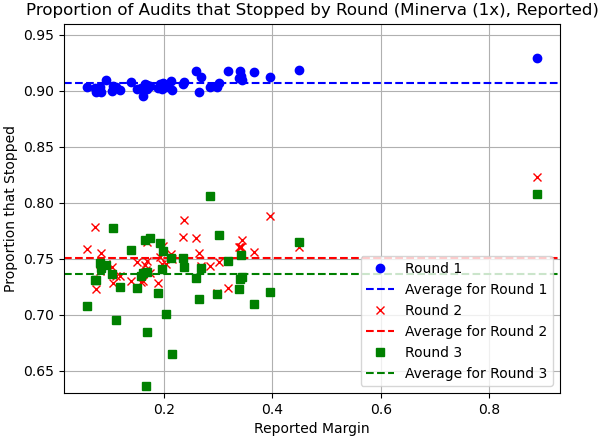
\includegraphics[width=0.5\textwidth]{scale/minerva1.png}
\pause 
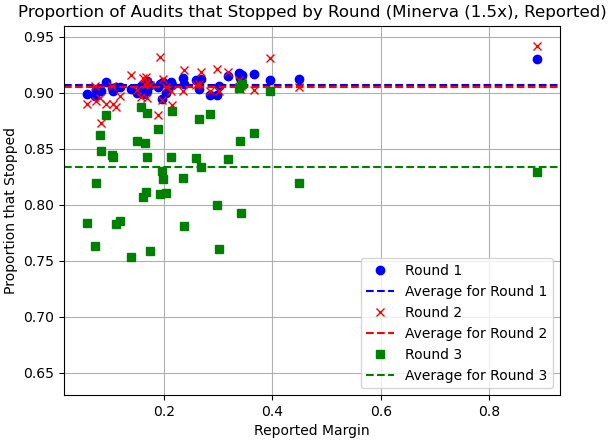
\includegraphics[width=0.5\textwidth]{scale/minerva1p5.png}
\end{frame}

\begin{frame}
\frametitle{Results: Stopping Probability ($\chi_1=0.25$)}

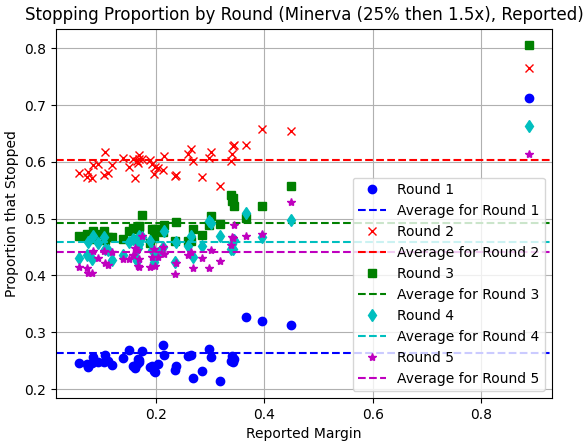
\includegraphics[width=1\textwidth]{minerva25percthen1p5_sprob.png}
\end{frame}


\begin{frame}
\frametitle{Results: Risk ($\chi_1=0.9$)}


\hspace{-.5cm} 
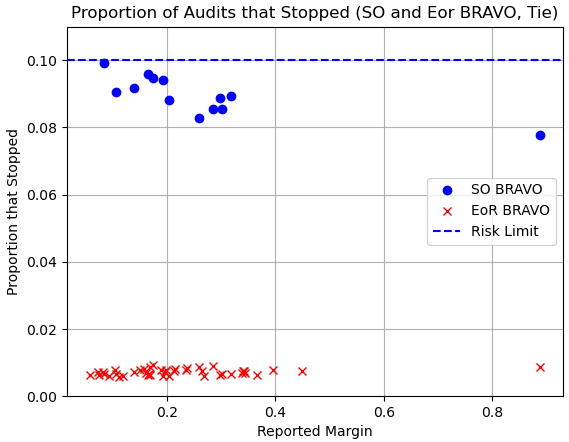
\includegraphics[width=.5\textwidth]{bravo_risks.png}
\pause 
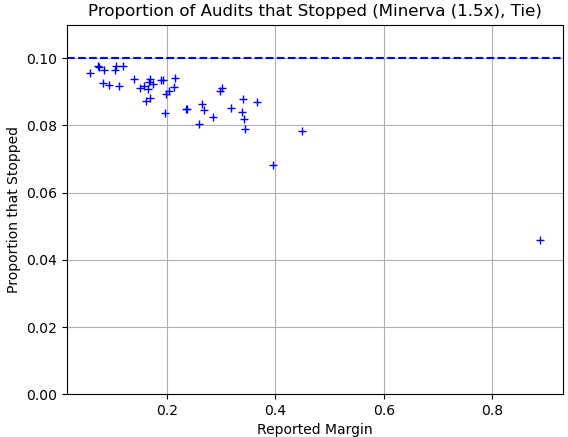
\includegraphics[width=.5\textwidth]{riskminerva1p5_10t4.png}

\end{frame}

\begin{frame}
\frametitle{Results: Number of Ballots ($\chi_1=0.9$)}
\centering

\pause 
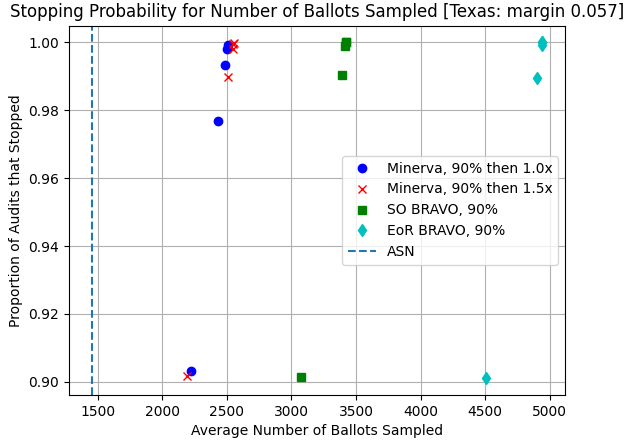
\includegraphics[width=1\textwidth]{texas90.png}
\end{frame}

\begin{frame}
\frametitle{Results: Number of Ballots ($\chi_1=0.25$)}

\centering
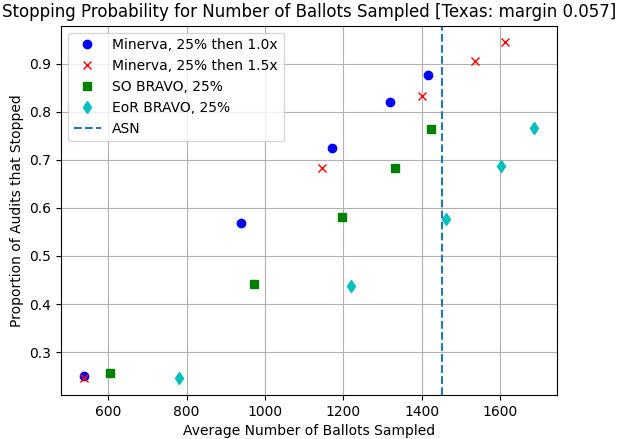
\includegraphics[width=1\textwidth]{texas25.png}
\end{frame}



\begin{frame}
\frametitle{Results: Round Size Proportions}

For $\chi_1 = 0.25$, the number of ballots required for \Minerva is smaller than that required by SO \BRAVO and EoR \BRAVO
\pause 
\begin{itemize}
\item Improvement considerably smaller than that when $\chi_1=0.9$
\pause 
\item SO \BRAVO: 
\begin{itemize}
\item for $\chi_1 =0.9$ requires a third more than does \Minerva
\item for $\chi_1 = 0.25$ requires a tenth more than does \Minerva
\end{itemize}
\pause 
\item EoR \BRAVO:
\begin{itemize}
\item for $\chi_1 = 0.9$ requires twice as many as \Minerva
\item for $\chi_1 =0.25$ requires a fourth to a half more (depending on margin) than does \Minerva
\end{itemize}

\end{itemize}
\end{frame}
\begin{frame}
\frametitle{Results: \Minerva Stopping Probabilities}


For $\chi_1 = 0.9$, \Minerva consequent conditional stopping probabilities for rounds two and three are respectively:
\begin{itemize} 
\pause
\item with multiplying factor $1$, $\chi_2\approx 0.75$ and $\chi_3\approx 0.74$
\pause
\item with multiplying factor $1.5$, $\chi_2\approx 0.91$ and $\chi_3\approx 0.83$
\end{itemize}

\end{frame}

\begin{frame}
\frametitle{Conclusion}

\begin{itemize}

\item We describe use of the R2B2 library and simulator to characterize: 
\begin{itemize}
\pause
\item maximum risk, 
\pause
\item stopping probability, and 
\pause
\item number of ballots 
\pause
\item for various round schedules.
\pause
\end{itemize}
\item \Minerva requires fewer ballots than either implementation of \BRAVO in all cases we study, but the advantage decreases for a smaller stopping probability for each round

\end{itemize}

\end{frame}

\begin{frame}
\frametitle{Future Work}
\begin{itemize}
\item More detailed study of the impact of different round schedules
\pause
\item Simulations with other underlying distributions
\end{itemize}
\end{frame}


\begin{frame}
\centering 
\bigskip
\bigskip
\bigskip
Thank you

\bigskip
\bigskip
\bigskip
\bigskip

odbroadrick@gmail.com
\end{frame}



% References?

\end{document}

